\documentclass{article}

%PACKAGE: math
\usepackage{amsmath}
%PACKAGE: figure
\usepackage{graphicx}
%PACKAGE: other
\usepackage{float}
%PACKAGE: table
\usepackage{booktabs} % For \toprule, \midrule and \bottomrule
\usepackage{siunitx} % Formats the units and values
\usepackage{pgfplotstable} % Generates table from .csv

%Setup siunitx
\sisetup{
  round-mode          = places, % Rounds numbers
  round-precision     = 2, % to 2 places
}

\title{Examples in Latex}
\date{2015-12}
\author{Mia Feng}

\begin{document}
	\pagenumbering{gobble}
	\maketitle
	\tableofcontents
	\newpage
	\pagenumbering{arabic}
	
	% Section
	\section{Section}
	I am a section.
	\subsection{subsection}
	I am a subsection.
	\paragraph{paragraph}
	I am a paragraph.
	\subparagraph{subparagraph}
	I am a subparagraph.
	
	% Math
	\section{Math}
	\subsection{Inline Math}
	Inline math $f(x) = x^2$ example.
	\subsection{Math Environments}
	\paragraph{Equation and Matrices}
	\begin{equation*}
		f(x) = x^2
	\end{equation*}
	\begin{equation}
		\left[
		\begin{matrix}
		1 & 0\\
		0 & 1
		\end{matrix}
		\right]
	\end{equation}
	
	\paragraph{Align}
	\begin{align*}
		f(x) &= x^2\\
		g(x) &= \frac{1}{x}\\
		F(x) &= \int^a_b 3\left(\frac{1}{\sqrt{x}}\right)
	\end{align*}
	
	% Figures
	\section{Figures}
	h!: here \newline
	H: need package float.
	\begin{figure}[H]
		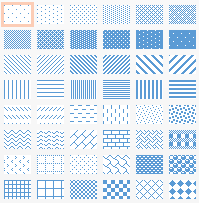
\includegraphics[scale=0.3]{Res/figure.png}
		\caption{Caption for the figure}
		\label{fig:fig1}
	\end{figure}
	
	% Tables
	\section{Tables}
	\subsection{A Table}
	\begin{table}[H]
		\centering
  		\caption{Caption for the table.}
		\label{tab:table1}
		\begin{tabular}{l|c||r}
			1 & 2 & 3\\
			\hline
			a & b & c\\
		\end{tabular}
	\end{table}
	\subsection{Using package booktabs}
	\begin{table}[h!]
		\centering
		\caption{Caption for the table.}
		\label{tab:table2}
		\begin{tabular}{ccc}
			\toprule
			some & actual & content\\
			\midrule
			first & content & row\\
			second & content & row\\
			\bottomrule
		\end{tabular}
	\end{table}
	\subsection{CSV Table}
	Setup siunitx at the beginning.
	\begin{table}[h!]
 	 \begin{center}
    \caption{Autogenerated table from .csv file.}
    \label{tab:table3}
    \pgfplotstabletypeset[
      multicolumn names, % allows to have multicolumn names
      col sep=comma, % the seperator in our .csv file
      display columns/0/.style={
		column name=$Value 1$, % name of first column
		column type={S},string type},  % use siunitx for formatting
      display columns/1/.style={
		column name=$Value 2$,
		column type={S},string type},
	display columns/2/.style={
		column name=$Value 3$,
		column type={S},string type},
      every head row/.style={
		before row={\toprule}, % have a rule at top
		after row={
			\si{\ampere} & \si{\volt} & \si{\volt} \\ % the units seperated by &
			\midrule} % rule under units
			},
		every last row/.style={after row=\bottomrule}, % rule at bottom
    ]{Res/table.csv} % filename/path to file
  \end{center}
\end{table}
	
	% Citation
	\section{Citation}
	This book is cited, see reference \cite{REF:1}.

	\newpage
	
	\bibliography{Res/Bib}
	\bibliographystyle{ieeetr}
	
	\newpage
	\begin{appendix}
		\listoffigures
		\listoftables
	\end{appendix}
\end{document}

